% -*- fill-column: 52 -*-
% (local-set-key (kbd "C-c C-f") 'display-fill-column-indicator-mode)

\chapter{Ismerkedés}

Az első leckében egy családfa vizsgálatán keresztül
megismerkedünk a programok alkotóelemeivel és a
\emph{rekurzió}\/val.

\section{Tények}

Egy Prolog program \emph{tényekből} és
\emph{szabályokból} áll, amelyekből a számítógép
következtetéseket tud levonni. Ha megadunk egy tény-
és szabályrendszert, utána kérdéseket tehetünk fel,
amelyeket a gép legjobb tudása szerint megválaszol.

Példaként vegyük Mohamed próféta családját
(\ref{fig:csaladfa}.~ábra)!
%
\begin{figure}
  \centering
  \begin{tikzpicture}
    \gtrset{edges={foreground={line width=2pt,black},no background}}
    \genealogytree[template=signpost,
                   options for node=m{box={colback=blue!20}},
                   options for family={af}{extra edges=ta{foreground={line width=2pt,black}}}]{
      child {
        g[male,phantom]{Valaki}
        c[male,id=t]{\large Abú Tálib}
        child[id=af] {
          g[male]{\large Abdulla}
          p[female]{\large Ámna}
          child {
            g[male,id=m]{\large Mohamed}
            p[female]{\large Hadídzsa}
            child {
              p[male,id=a]{\large Ali}
              g[female]{\large Fátima}
              c[male]{\large Huszajn}
              c[male]{\large Muhszin}
              c[male]{\large Haszan}
            }
            child {
              g[female]{\large Zajnab}
              c[female]{\large Umáma}
            }
          }
        }
      }
    }
  \end{tikzpicture}
  \caption{Mohamed próféta családja (részlet).}
  \label{fig:csaladfa}
\end{figure}
%
A szülő--gyerek kapcsolatokat az alábbi program
foglalja össze:

\begin{program}
szülő(abú_tálib, ali).
szülő(abdulla, mohamed).
szülő(ámna, mohamed).
szülő(mohamed, fátima).
szülő(hadídzsa, fátima).
szülő(mohamed, zajnab).
szülő(hadídzsa, zajnab).
szülő(ali, huszajn).
szülő(fátima, huszajn).
szülő(ali, muhszin).
szülő(fátima, muhszin).
szülő(ali, haszan).
szülő(fátima, haszan).
szülő(zajnab, umáma).
\end{program}

Ebben a programban minden sor egy \emph{tény}. Egy
tény dolgok (itt emberek) közti kapcsolatot ír le. A
formája a következő: a kapcsolat nevével kezdődik
(most ez a \pr{szülő}), utána zárójelek között
vesszővel elválasztva felsoroljuk a kapcsolatban
levő dolgokat, és a végén egy ponttal (\pr{.})
zárjuk.\index{teny@tény}

Talán furcsa lehet, hogy minden kisbetűvel van --
majd később lesz szó arról, hogy mik az elnevezés
pontos szabályai, egyelőre azt jegyezzük meg, hogy
minden \emph{konkrét} dolog kisbetűvel írandó, és
nem lehet benne szóköz.

\begin{infobox}{}{Mohamed családfája}
A programban a családfának csak egy nagyon kis
szeletét használtuk, és még ezen a részen belül
sem tartalmaz minden kapcsolatot, mert pl.~Ali
Fátima halála után feleségül vette Umámát is.

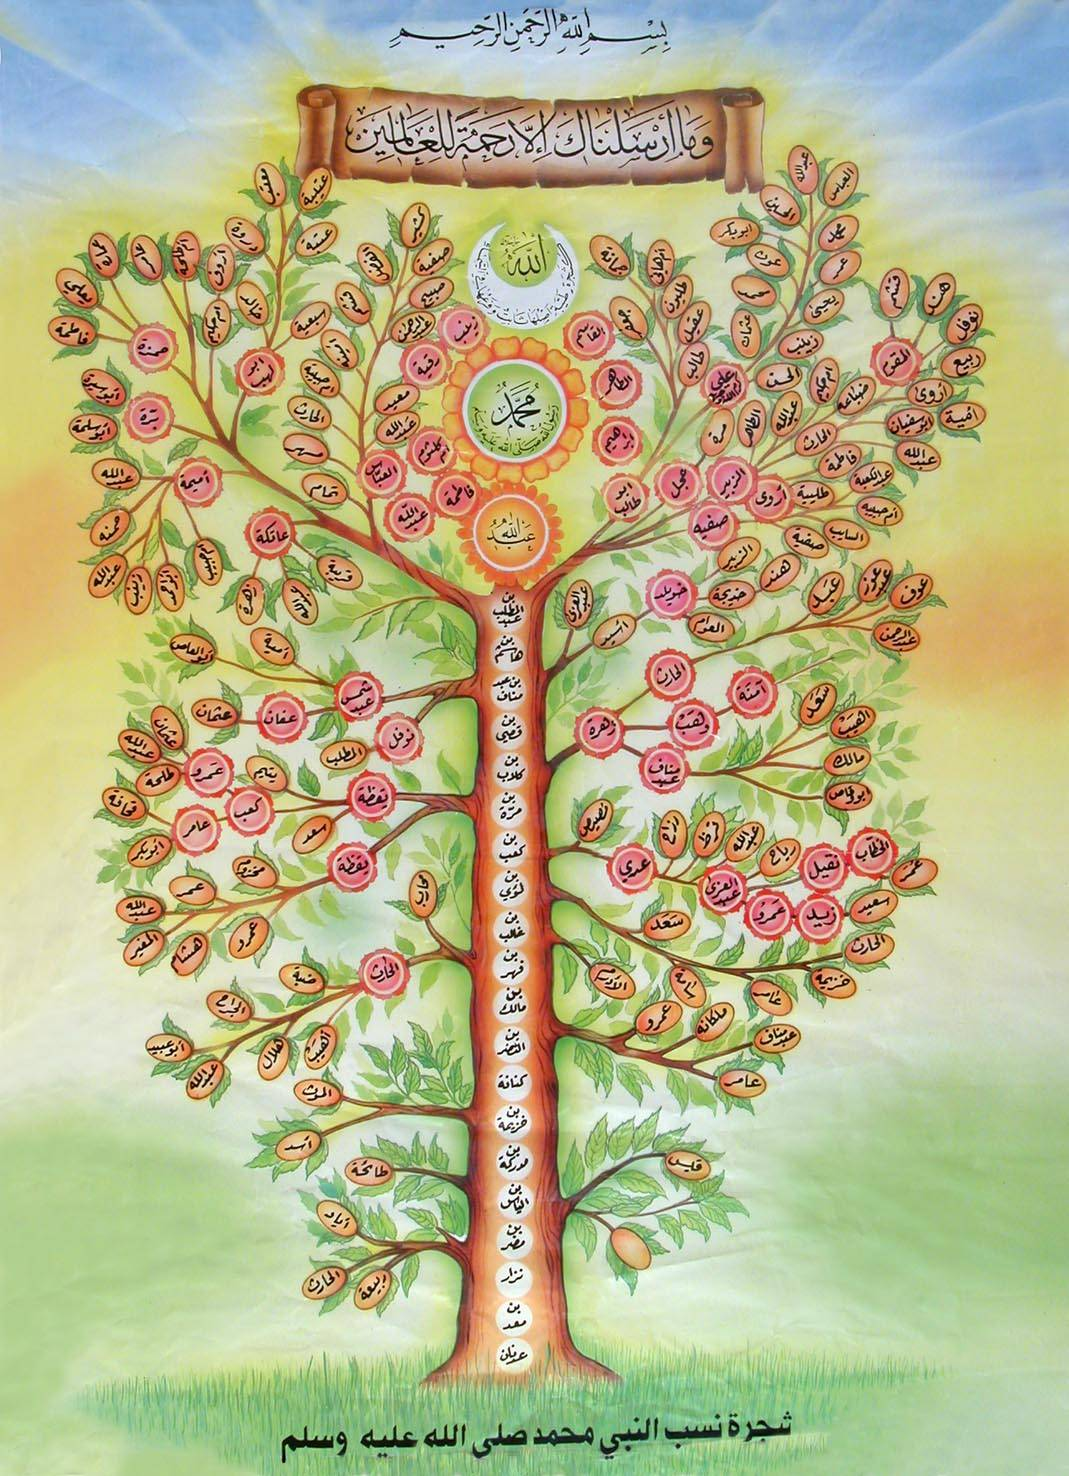
\includegraphics[width=\textwidth]{images/prophet-family.jpg}
\end{infobox}

\subsection*{Egyszerű kérdések}

Már egy ilyen egyszerű program esetén is lehet
értelmes kérdéseket feltenni. Például
megkérdezhetjük, hogy
\begin{query}
?- szülő(mohamed, fátima).
\end{query}
\dots amire a rendszer a \pr{true} (igaz) vagy
\pr{yes} (igen) üzenettel
válaszol;\index{\pr{true}}\index{\pr{yes}} vagy hogy
\begin{query}
?- szülő(ali, zajnab).
\end{query}
\dots amire a \pr{false} (hamis) vagy \pr{no} (nem)
eredményt adja.\index{\pr{false}}\index{\pr{no}} (A
továbbiakban ez a könyv a \pr{true} és \pr{false}
válaszokat fogja használni.)

Egy kicsit érdekesebb a következő kérdés:
\begin{query}
?- szülő(mohamed, Kicsoda).
\end{query}
Erre azt a feleletet kapjuk, hogy \pr{Kicsoda =
  fátima}. Ha további válaszokat kérünk, akkor még
azt is kiírja alá, hogy \pr{Kicsoda = zajnab}.

Mi történt itt? Azáltal, hogy a második helyre egy
nagybetűs szót (\pr{Kicsoda}) írtunk, azt mondtuk,
hogy ez egy határozatlan, ismeretlen érték, egy
\emph{változó}.\index{valtozo@változó} A kérdést tehát
magyarul úgy lehetne megfogalmazni: ,,Mohamed kinek
a szülője?''

Erre megkeresi az első választ, amit talál
(\pr{fátima}), és ha továbbit kérünk tőle, akkor
megtalálja \pr{zajnab}ot is, és látja, hogy nincs
több, és így leáll.

Ha kisbetűvel írtuk volna:
\begin{query}
?- szülő(mohamed, kicsoda).
\end{query}
\dots akkor a \pr{false} eredményt kaptuk volna,
hiszen \pr{kicsoda} itt egy konkrét dolgot jelöl, a
kérdés tehát azt jelenti: ,,Igaz-e, hogy Mohamed
szülője Kicsodának?''

A kérdés a másik irányban is feltehető:
\begin{query}
?- szülő(Ki, ali).
\end{query}
\dots tehát ,,Ki Ali szülője?'', amire a \pr{Ki =
  abú\_tálib} feleletet kapjuk.

Még tovább is mehetünk, és rákérdezhetünk az összes
szülő-gyerek kapcsolatra:
\begin{query}
?- szülő(Ki, Kinek).
\end{query}
\dots azaz ,,Ki kinek a szülője?''. Az első válasz
az lesz, hogy
\begin{query}
Ki = abú_tálib,
Kinek = ali
\end{query}
További válaszok kérésével sorban megkapjuk az
adatbázisunk minden egyes elemét.

\subsection*{Összetett kérdések}

Tegyük fel, hogy arra vagyunk kíváncsiak, hogy kik
Mohamed unokái. Hogyan tudjuk ezt megkérdezni? Az
unoka definíció szerint a gyerek gyereke, tehát
tudjuk, hogy van valaki, aki szülője az unokának, és
akinek a szülője Mohamed. A logikai \emph{és}\/sel
összekötött, együtt teljesítendő feltételeket
vesszővel választjuk el:
\begin{query}
?- szülő(mohamed, Valaki), szülő(Valaki, Unoka).
\end{query}
Négy megoldást is kapunk:
\begin{query}
Unoka = huszajn,
Valaki = fátima
Unoka = muhszin,
Valaki = fátima
Unoka = haszan,
Valaki = fátima
Unoka = umáma,
Valaki = zajnab
\end{query}
(Ezek páronként értendők, tehát Fátimától van
Huszajn, Muhszin és Haszan, és Zajnabtól Umáma.)

Ez azért működik, mert egy változónak minden
előfordulása azonos értéket kell, hogy kapjon.
A kérdés két tagjának sorrendje felcserélhető, tehát
ugyanezt az eredményt adja ez is:
\begin{query}
?- szülő(Valaki, Unoka), szülő(mohamed, Valaki).
\end{query}
(Majd látni fogjuk viszont, hogy a számításigényük
nem azonos, érdemesebb az erősebb megszorítással
kezdeni.)

Hasonlóan rákérdezhetünk, hogy kik Huszajn
nagyszülei:
\begin{query}
?- szülő(Valaki, huszajn), szülő(Nagyszülő, Valaki).
\end{query}
\dots amire megkapjuk Abú Tálibot, Mohamedet és
Hadídzsát.

Ha arra vagyunk kíváncsiak, hogy Haszan testvére-e
Huszajnnak, így fogalmazhatjuk meg:
\begin{query}
?- szülő(Valaki, haszan), szülő(Valaki, huszajn).
\end{query}
Azt kapjuk, hogy \pr{Valaki = ali}, tehát a válasz
igen. Ha \pr{huszajn} helyett \pr{abdullá}t írunk,
akkor \pr{false} választ kapunk.

\begin{problem}
Válaszold meg az alábbi kérdéseket!
\begin{query}
?- szülő(huszajn, X).
?- szülő(X, huszajn).
?- szülő(ámna, X), szülő(X, fátima).
?- szülő(ámna, X), szülő(X, Y), szülő(Y, haszan).
\end{query}
\end{problem}
\begin{problem}
Fogalmazd meg Prologban!
\begin{enumerate}
\item Ki Ali szülője?
\item Umámának van gyereke?
\item Ki Zajnab nagyszülője?
\end{enumerate}
\end{problem}
\begin{problem}
Készítsd el a saját családfádat (nagyszülőkig
és unokatestvérekig)!
\end{problem}

\section{Szabályok}

Eddig csak tényekkel foglalkoztunk, de valójában a
Prolog programok nagy része \emph{szabályokból}
áll. Először is egészítsük ki a programunkat a
szereplőink nemével!\index{szabály}

\begin{program}
férfi(abú_tálib).
férfi(abdulla).
férfi(mohamed).
férfi(ali).
férfi(huszajn).
férfi(muhszin).
férfi(haszan).

nő(ámna).
nő(hadídzsa).
nő(fátima).
nő(zajnab).
nő(umáma).
\end{program}

Ha most a \pr{szülő} mellett szeretnénk \pr{anya} és
\pr{apa} kapcsolatokat is létrehozni, ezt
megtehetjük egyenként:
\begin{program}
anya(ámna, mohamed).
anya(hadídzsa, fátima).
...
apa(abú_tálib, ali).
apa(abdulla, mohamed).
...
\end{program}
Ez azonban elég sok munka, és érezzük, hogy
felesleges, hiszen kikövetkeztethető.  Szabályok
segítségével ezt sokkal egyszerűbben megoldhatjuk:
\begin{program}
anya(X, Y) :- szülő(X, Y), nő(X).
apa(X, Y) :- szülő(X, Y), férfi(X).
\end{program}
A \pr{:-} jelet itt úgy olvashatjuk ki, hogy
,,akkor, ha'', tehát ,,X anyja Y-nak akkor, ha X
szülője Y-nak és X nő''. A baloldalon levő részt a
szabály \emph{fej}\/ének, a jobboldalát a szabály
\emph{törzs}\/ének nevezzük.
\index{\pr{:-}}\index{fej}\index{torzs@törzs}

Mi történik, amikor feltesszük az alábbi kérdést?
\begin{query}
?- anya(ámna, mohamed).
\end{query}
A rendszer megtalálja az \pr{anya} szabályt, és
\emph{egyesíti} az \pr{X}-et \pr{ámná}\-val, az
\pr{Y}-t pedig \pr{mohamed}del.\index{egyesítés} (Az
egyesítésről még később szó lesz, itt egyszerűen
helyettesítést jelent.) Ezután megnézi, hogy a
szabály jobboldalán levő feltétel teljesül-e; ez
most a
\begin{query}
szülő(ámna, mohamed), nő(ámna).
\end{query}
\dots és ezek a tények szerepelnek a programban,
tehát \pr{true} válasszal tér vissza.

Definiáljuk a ,,nagyszülő'' kapcsolatot!
\begin{program}
nagyszülő(X, Z) :- szülő(X, Y), szülő(Y, Z).
\end{program}
Ez pontosan követi azt, ahogy megkerestük valakinek
a nagyszülőjét.

\subsection*{Problémás esetek}

Hogyan tudnánk megadni a ,,fivér'' kapcsolatot?
\begin{program}
fivér(X, Y) :- férfi(X), szülő(Z, X), szülő(Z, Y).
\end{program}
Tehát X fivére Y-nak, ha férfi és van közös
szülőjük.

Itt érdemes megjegyezni, hogy bár Abú Tálib és
Abdulla testvérek voltak, a
\begin{query}
?- fivér(abú_tálib, abdulla).
\end{query}
kérdésre \pr{false} a válasz, mivel a programnak
nincs arról tudomása, hogy lenne közös szülőjük. (A
Prolog mindent hamisnak vesz, amit az általa ismert
adatokból nem tud kikövetkeztetni, és ez időnként
furcsa következményekkel járhat -- erről majd
később.)

Egy másik problémába ütközünk, ha Mohamed fivéreire
vagyunk kíváncsiak:
\begin{query}
?- fivér(mohamed, X).
\end{query}
Az eredmény, meglepő módon, \pr{X = mohamed}! Ebből
látszik, hogy a definíciónk nem volt elég pontos;
hozzá kell venni azt is, hogy senki nem fivére
önmagának:
\begin{program}
fivér(X, Y) :-
    férfi(X),
    szülő(Z, X), szülő(Z, Y),
    X \= Y.
\end{program}
Itt a \pr{\textbackslash=} jelentése ,,nem azonos''.
\index{\pr{\textbackslash=}} Ez a példa azt is
illusztrálja, hogy a szabályok több sorban is
írhatóak; ilyenkor a második és további sorokat
beljebb szokás húzni.

\subsection*{Egyedüli változók}

Készítsük el a
\begin{program}
vangyereke(X) :- szülő(X, Y).
\end{program}
szabályt.  Ennek az az érdekessége, hogy attól
függően, hogy hogyan olvassuk ki, az állítás
\emph{minden} Y-ra vonatkozik, vagy csak azt
mondja, hogy \emph{létezik} egy fajta Y:

\begin{enumerate}
\item (Minden X és Y esetén,) ha X szülője Y-nak,
  akkor X-nek van gyereke.
\item X-nek akkor van gyereke, ha létezik olyan Y,
  hogy X szülője Y-nak.
\end{enumerate}
A két olvasat egyenértékű; ez a kettősség annak a
következménye, hogy az \pr{Y} változó csak a szabály
törzsében fordul elő.

A fenti példa más miatt is érdekes. Mivel az \pr{Y}
változó a szabályban mindössze egyszer fordul elő,
nem lehet hatással az eredmény kiszámítására, tehát
érdektelen. Ezt úgy szokás jelezni, hogy a helyére
egy alsóvonást (\pr{\_}) írunk, vagy egy ezzel
kezdődő nevet (pl.~\pr{\_Y}).\index{\pr{\_}} Ha
kérdésben szerepel ilyen változó, akkor a válaszban
ennek az értéke nem fog megjelenni. Így pl.~az
alábbi kérdés megadja Mohamed unokáit anélkül, hogy
megmutatná a szülőket:
\begin{query}
?- szülő(mohamed, _Valaki), szülő(_Valaki, Unoka).
\end{query}

Ha több alsóvonás szerepel, ezek értéke lehet
különböző, tehát a
\begin{query}
?- szülő(_, _).
\end{query}
kérdésre \pr{true} lesz a válasz, pedig senki sem
szülője önmagának.

Ha egy egyszer szereplő változónak ,,normális''
nevet adunk, akkor erre a fordító általában
figyelmeztet minket, mert ez gyakran egy elírás
következménye. Pl.~az alábbi programban a
\pr{Valaki} változóból egyszer kimaradt egy \pr{a}
betű:
\begin{program}
nagyszülő(X, Y) :-
    szülő(X, Valaki), szülő(Valki, Y).
\end{program}

\begin{problem}
Fordítsd le Prologra!
\begin{enumerate}  
\item Akinek van gyereke, az boldog. (\pr{boldog}
  szabály)
\item Minden X-re, ha X-nek van egy gyereke akinek
  van egy fivére, akkor X-nek két gyereke
  van. (\pr{kétgyerekes} szabály)
\end{enumerate}
\end{problem}
\begin{problem}
  Készítsd el az \pr{unoka} szabályt!
  Teszteld a saját családfádon!
\end{problem}
\begin{problem}
  Csinálj egy \pr{nagybácsi} szabályt a \pr{szülő}
  és \pr{fivér} segítségével, és keresd meg vele Ali
  unokahúgait!
\end{problem}

\section{Rekurzív szabályok}
Adjunk még egy utolsó szabályt a programunkhoz: az
\emph{ős} fogalmát. Valakinek az őseit úgy kapjuk
meg, hogy felfelé megyünk a családfában: ős a szülő,
a nagyszülő, a dédszülő stb. Ezt elkezdhetjük írni
szabályokkal:
\begin{program}
ős(X, Z) :- szülő(X, Z).
ős(X, Z) :- szülő(X, Y), szülő(Y, Z).
ős(X, Z) :-
    szülő(X, Y1), szülő(Y1, Y2), szülő(Y2, Z).
ős(X, Z) :-
    szülő(X, Y1), szülő(Y1, Y2),
    szülő(Y2, Y3), szülő(Y3, Z).
...
\end{program}
Ez nagyon jól működik, de véges -- bármennyi ilyen
programsort írok, mindig tudok eggyel feljebb menni
a családfában, és azt már nem kezeli.

Egy kis trükkel meg tudjuk ezt oldani: azt mondjuk,
hogy ha X gyereke őse Z-nek, akkor X is őse Z-nek:
\begin{program}
ős(X, Z) :- szülő(X, Y), ős(Y, Z).
\end{program}
Az \pr{ős} így önmagára hivatkozik, más szóval
\emph{rekurzív}.\index{rekurzió}

Ez így magában még azonban nem elég, mert így ahhoz,
hogy valaki ős legyen, mindig valaki másnak is ősnek
kéne lennie, valahol ennek meg kéne állnia. Elég
hozzávenni a legegyszerűbb esetet, amikor a szülő az
ős:
\begin{program}
ős(X, Z) :- szülő(X, Z).
ős(X, Z) :- szülő(X, Y), ős(Y, Z).
\end{program}
Ez a kettő együtt már működik. X őse Z-nek, ha vagy
(i) X szülője Z-nek, vagy (ii) X szülője Y-nak és Y
őse Z-nek. Próbáljátok ki, mit ad az
\begin{query}
?- ős(X, huszajn).
\end{query}
kérdés!

\begin{problem}
Tegyük fel, hogy az \pr{ős} definícióját
megváltoztatjuk!
\begin{program}
ős(X, Z) :- szülő(X, Z).
ős(X, Z) :- szülő(Y, Z), ős(X, Y).
\end{program}
Jó ez így? Miért?
\end{problem}

\section*{A teljes program}

Itt van minden tény és szabály, amiről szó volt. A
programban a \pr{\%} jel megjegyzések hozzáadására
használható, a rendszer szempontjából a \pr{\%}-tól
jobbra levő szöveg érdektelen, mintha ott se
lenne.

\begin{program}
% szülő(X, Y) => X az Y szülője
szülő(abú_tálib, ali).
szülő(abdulla, mohamed).
szülő(ámna, mohamed).
szülő(mohamed, fátima).
szülő(hadídzsa, fátima).
szülő(mohamed, zajnab).
szülő(hadídzsa, zajnab).
szülő(ali, huszajn).
szülő(fátima, huszajn).
szülő(ali, muhszin).
szülő(fátima, muhszin).
szülő(ali, haszan).
szülő(fátima, haszan).
szülő(zajnab, umáma).

férfi(abú_tálib).
férfi(abdulla).
férfi(mohamed).
férfi(ali).
férfi(huszajn).
férfi(muhszin).
férfi(haszan).

nő(ámna).
nő(hadídzsa).
nő(fátima).
nő(zajnab).
nő(umáma).

anya(X, Y) :- szülő(X, Y), nő(X).   % X az Y anyja
apa(X, Y) :- szülő(X, Y), férfi(X). % X az Y apja

nagyszülő(X, Z) :- szülő(X, Y), szülő(Y, Z).

fivér(X, Y) :-
    férfi(X),
    szülő(Z, X), szülő(Z, Y),
    X \= Y.

vangyereke(X) :- szülő(X, _).

ős(X, Z) :- szülő(X, Z).
ős(X, Z) :- szülő(X, Y), ős(Y, Z).
\end{program}

\clearpage

\section{Projekt: a négyszín-tétel}
Mindössze négy szín elég ahhoz, hogy tetszőleges
térképen az országokhoz színeket rendeljünk úgy,
hogy minden országhatár két különböző színt
válasszon el. (Ez feltételezi, hogy az országok
mindig összefüggőek, tehát nincsen másik ország, ami
kettéválasztaná őket -- ez egy valódi térképnél
gyakran nem teljesül.)

Próbáljuk meg kiszínezni Európa egy szeletét!

\begin{center}
  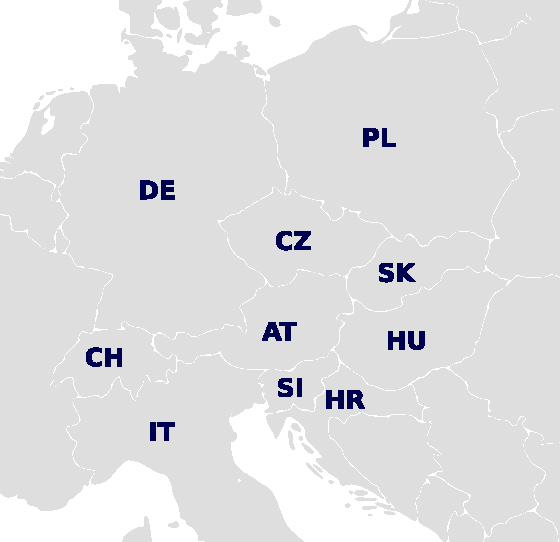
\includegraphics[width=0.7\textwidth]{images/europe.pdf}
\end{center}

Jelölje \pr{t} azt, hogy két ország
\emph{találkozik}. A találkozáskor a színeknek
különbözőeknek kell lennie, tehát felvehetjük a
következő tényeket (egyelőre 2 színnel):
\begin{program}
t(piros, zöld). t(zöld, piros).
\end{program}
Ahhoz, hogy a térképünk megfeleljen a
követelményeknek, minden határnál teljesülnie kell
egy ilyen találkozásnak:
\begin{program}
térkép(DE, CH, IT, PL, CZ, AT, SI, HR, SK, HU) :-
    t(DE, PL), t(DE, CZ), t(DE, AT), t(DE, CH),
    t(CH, AT), t(CH, IT),
    t(IT, AT), t(IT, SI),
    t(PL, CZ), t(PL, SK),
    t(CZ, AT), t(CZ, SK),
    t(AT, SK), t(AT, HU), t(AT, SI),
    t(SI, HU), t(SI, HR),
    t(HR, HU),
    t(SK, HU).
\end{program}

\begin{infobox}{}{a négyszín-tétel}
Ez volt az első olyan matematikai tétel, amelynek
bizonyítását számítógéppel adták meg, és ezért sok
matematikus kezdetben nem is fogadta el
bizonyítottnak, és csak ,,négyszín-sejtésként''
hivatkoztak rá. Minden joguk megvolt rá: a több,
mint egy hónapon át futó 1976-os eredeti program
állítólag tele volt hibákkal. 20 évvel később
azonban egy sokkal hatékonyabb megoldást is
találtak, és 2004-ben egy tételbizonyító rendszer is
belátta, hogy az állítás mindig igaz.
\end{infobox}

Mivel a színekre vonatkozó szabályt mindkét
sorrendben felvettük, az országok sorrendje nem
számít, és így elég mindig csak az egyik verziót
felírni. Ha most megkérdezzük, hogy
\begin{query}
?- térkép(DE, CH, IT, PL, CZ, AT, SI, HR, SK, HU).
\end{query}
\dots akkor (nem túl meglepő módon) tagadó választ
kapunk. Vegyünk hozzá még egy színt!
\begin{program}
t(piros, kék). t(zöld, kék).
t(kék, piros). t(kék, zöld).
\end{program}
\dots még mindig nem elég. (Ez is elég világos -- ha
Ausztria pl.~piros, akkor a szomszédos országokat
körbejárva felváltva kéne zöldet és kéket kapnunk,
de páratlan számú ország van körülötte.)
Vegyük akkor hozzá a sárgát is!
\begin{program}
t(piros, sárga). t(zöld, sárga). t(kék, sárga).
t(sárga, piros). t(sárga, zöld). t(sárga, kék).
\end{program}
Ha most tesszük fel a kérdést, akkor már talál
megoldást:
\begin{query}
AT = PL = zöld,
CH = CZ = SI = kék,
DE = HR = IT = SK = piros,
HU = sárga
\end{query}
Az egyetlen szépséghibája, hogy Szlovénia kék lett,
és így egybefolyhat a tenger kékjével. Több
lehetőségünk is van:
\begin{itemize}
\item Lecseréljük a kéket egy másik színre
\item Addig kérünk további megoldásokat, amíg már
  egy tengerparti ország sem lesz kék színű
\item Felcseréljük a kék és sárga színeket
\end{itemize}

Tegyük fel, hogy szeretjük a kék színt, és nem
akarjuk lecserélni (meg egyébként is akkor már 5
szín kéne!), a másik két megoldás pedig nem elég
automatikus. Mit tehetünk?

Felvehetjük plusz ,,országként'' a tengert, és
megkövetelhetjük, hogy mindig kék legyen:
\begin{program}
térkép(DE, CH, IT, PL, CZ, AT, SI, HR, SK, HU) :-
    Tenger = kék,
    t(DE, PL), t(DE, CZ), t(DE, AT), t(DE, CH),
    t(CH, AT), t(CH, IT),
    t(IT, AT), t(IT, SI),
    t(PL, CZ), t(PL, SK),
    t(CZ, AT), t(CZ, SK),
    t(AT, SK), t(AT, HU), t(AT, SI),
    t(SI, HU), t(SI, HR),
    t(HR, HU),
    t(SK, HU),
    t(DE, Tenger), t(IT, Tenger), t(PL, Tenger),
    t(SI, Tenger), t(HR, Tenger).
\end{program}
Így már tökéletes megoldást kapunk.

Megtehettük volna azt is, hogy a \pr{Tenger}ek
helyett egyszerűen \pr{kék}et írunk, és akkor
nincsen szükség a \pr{Tenger = kék} sorra sem, de
egy kicsit kevésbé olvasható lenne a
forráskód. Ilyen rövid programoknál még ez nem olyan
lényeges, de általában a programozásban fontos arra
törekedni, hogy ne csak a számítógép, hanem egy
másik ember (és pár hét múlva mi magunk) is
megértse, amit írtunk.
